\documentclass{ximera}

%\usepackage{todonotes}

\newcommand{\todo}{}

\usepackage{tkz-euclide}
\tikzset{>=stealth} %% cool arrow head
\tikzset{shorten <>/.style={ shorten >=#1, shorten <=#1 } } %% allows shorter vectors

\usepackage{tkz-tab}  %% sign charts
\usetikzlibrary{decorations.pathreplacing} 

\usetikzlibrary{backgrounds} %% for boxes around graphs
\usetikzlibrary{shapes,positioning}  %% Clouds and stars
\usetikzlibrary{matrix} %% for matrix
\usepgfplotslibrary{polar} %% for polar plots
\usetkzobj{all}
\usepackage[makeroom]{cancel} %% for strike outs
%\usepackage{mathtools} %% for pretty underbrace % Breaks Ximera
\usepackage{multicol}

\usepackage{polynom}



\usepackage[many]{tcolorbox}  %% for titled boxes
\newtcolorbox{xbox}[1]{%
    tikznode boxed title,
    enhanced,
    arc=0mm,
    interior style={white},
    attach boxed title to top center= {yshift=-\tcboxedtitleheight/2},
    fonttitle=\bfseries,
    colbacktitle=white,coltitle=black,
    boxed title style={size=normal,colframe=white,boxrule=0pt},
    title={#1}}


\usepackage{array}
\setlength{\extrarowheight}{+.1cm}   
\newdimen\digitwidth
\settowidth\digitwidth{9}
\def\divrule#1#2{
\noalign{\moveright#1\digitwidth
\vbox{\hrule width#2\digitwidth}}}





\newcommand{\RR}{\mathbb R}
\newcommand{\R}{\mathbb R}
\newcommand{\N}{\mathbb N}
\newcommand{\Z}{\mathbb Z}

%\renewcommand{\d}{\,d\!}
\renewcommand{\d}{\mathop{}\!d}
\newcommand{\dd}[2][]{\frac{\d #1}{\d #2}}
\newcommand{\pp}[2][]{\frac{\partial #1}{\partial #2}}
\renewcommand{\l}{\ell}
\newcommand{\ddx}{\frac{d}{\d x}}
\newcommand{\ddt}{\frac{d}{\d t}}

\newcommand{\zeroOverZero}{\ensuremath{\boldsymbol{\tfrac{0}{0}}}}
\newcommand{\inftyOverInfty}{\ensuremath{\boldsymbol{\tfrac{\infty}{\infty}}}}
\newcommand{\zeroOverInfty}{\ensuremath{\boldsymbol{\tfrac{0}{\infty}}}}
\newcommand{\zeroTimesInfty}{\ensuremath{\small\boldsymbol{0\cdot \infty}}}
\newcommand{\inftyMinusInfty}{\ensuremath{\small\boldsymbol{\infty - \infty}}}
\newcommand{\oneToInfty}{\ensuremath{\boldsymbol{1^\infty}}}
\newcommand{\zeroToZero}{\ensuremath{\boldsymbol{0^0}}}
\newcommand{\inftyToZero}{\ensuremath{\boldsymbol{\infty^0}}}



\newcommand{\numOverZero}{\ensuremath{\boldsymbol{\tfrac{\#}{0}}}}
\newcommand{\dfn}{\textbf}
%\newcommand{\unit}{\,\mathrm}
\newcommand{\unit}{\mathop{}\!\mathrm}
\newcommand{\eval}[1]{\bigg[ #1 \bigg]}
\newcommand{\seq}[1]{\left( #1 \right)}
\renewcommand{\epsilon}{\varepsilon}
\renewcommand{\iff}{\Leftrightarrow}

\DeclareMathOperator{\arccot}{arccot}
\DeclareMathOperator{\arcsec}{arcsec}
\DeclareMathOperator{\arccsc}{arccsc}
\DeclareMathOperator{\si}{Si}
\DeclareMathOperator{\proj}{proj}
\DeclareMathOperator{\scal}{scal}


\newcommand{\tightoverset}[2]{% for arrow vec
  \mathop{#2}\limits^{\vbox to -.5ex{\kern-0.75ex\hbox{$#1$}\vss}}}
\newcommand{\arrowvec}[1]{\tightoverset{\scriptstyle\rightharpoonup}{#1}}
\renewcommand{\vec}{\mathbf}
\newcommand{\veci}{\vec{i}}
\newcommand{\vecj}{\vec{j}}
\newcommand{\veck}{\vec{k}}
\newcommand{\vecl}{\boldsymbol{\l}}

\newcommand{\dotp}{\bullet}
\newcommand{\cross}{\boldsymbol\times}
\newcommand{\grad}{\boldsymbol\nabla}
\newcommand{\divergence}{\grad\dotp}
\newcommand{\curl}{\grad\cross}
%\DeclareMathOperator{\divergence}{divergence}
%\DeclareMathOperator{\curl}[1]{\grad\cross #1}


\colorlet{textColor}{black} 
\colorlet{background}{white}
\colorlet{penColor}{blue!50!black} % Color of a curve in a plot
\colorlet{penColor2}{red!50!black}% Color of a curve in a plot
\colorlet{penColor3}{red!50!blue} % Color of a curve in a plot
\colorlet{penColor4}{green!50!black} % Color of a curve in a plot
\colorlet{penColor5}{orange!80!black} % Color of a curve in a plot
\colorlet{fill1}{penColor!20} % Color of fill in a plot
\colorlet{fill2}{penColor2!20} % Color of fill in a plot
\colorlet{fillp}{fill1} % Color of positive area
\colorlet{filln}{penColor2!20} % Color of negative area
\colorlet{fill3}{penColor3!20} % Fill
\colorlet{fill4}{penColor4!20} % Fill
\colorlet{fill5}{penColor5!20} % Fill
\colorlet{gridColor}{gray!50} % Color of grid in a plot

\newcommand{\surfaceColor}{violet}
\newcommand{\surfaceColorTwo}{redyellow}
\newcommand{\sliceColor}{greenyellow}




\pgfmathdeclarefunction{gauss}{2}{% gives gaussian
  \pgfmathparse{1/(#2*sqrt(2*pi))*exp(-((x-#1)^2)/(2*#2^2))}%
}


%%%%%%%%%%%%%
%% Vectors
%%%%%%%%%%%%%

%% Simple horiz vectors
\renewcommand{\vector}[1]{\left\langle #1\right\rangle}


%% %% Complex Horiz Vectors with angle brackets
%% \makeatletter
%% \renewcommand{\vector}[2][ , ]{\left\langle%
%%   \def\nextitem{\def\nextitem{#1}}%
%%   \@for \el:=#2\do{\nextitem\el}\right\rangle%
%% }
%% \makeatother

%% %% Vertical Vectors
%% \def\vector#1{\begin{bmatrix}\vecListA#1,,\end{bmatrix}}
%% \def\vecListA#1,{\if,#1,\else #1\cr \expandafter \vecListA \fi}

%%%%%%%%%%%%%
%% End of vectors
%%%%%%%%%%%%%

%\newcommand{\fullwidth}{}
%\newcommand{\normalwidth}{}



%% makes a snazzy t-chart for evaluating functions
%\newenvironment{tchart}{\rowcolors{2}{}{background!90!textColor}\array}{\endarray}

%%This is to help with formatting on future title pages.
\newenvironment{sectionOutcomes}{}{} 



%% Flowchart stuff
%\tikzstyle{startstop} = [rectangle, rounded corners, minimum width=3cm, minimum height=1cm,text centered, draw=black]
%\tikzstyle{question} = [rectangle, minimum width=3cm, minimum height=1cm, text centered, draw=black]
%\tikzstyle{decision} = [trapezium, trapezium left angle=70, trapezium right angle=110, minimum width=3cm, minimum height=1cm, text centered, draw=black]
%\tikzstyle{question} = [rectangle, rounded corners, minimum width=3cm, minimum height=1cm,text centered, draw=black]
%\tikzstyle{process} = [rectangle, minimum width=3cm, minimum height=1cm, text centered, draw=black]
%\tikzstyle{decision} = [trapezium, trapezium left angle=70, trapezium right angle=110, minimum width=3cm, minimum height=1cm, text centered, draw=black]


\outcome{Understand what is meant by the form of a limit.}
\outcome{Calculate limits of the form zero over zero.}
\outcome{Identify determinate and indeterminate forms.}
\outcome{Distinguish between determinate and indeterminate forms.}
\outcome{Discuss why infinity is not a number.}

\title[Dig-In:]{Limits of the form zero over zero}

\begin{document}
\begin{abstract}
  We want to evaluate limits where the Limit Laws do not directly apply. 
\end{abstract}

\maketitle

In the last section, we were interested in the limits we could compute
using continuity and the limit laws. What about limits that cannot be
directly computed using these methods? Let's think about an example. Consider
\[
\lim_{x\to 2}\frac{x^2-3x+2}{x-2}.
\]
Here 
\[
\lim_{x\to 2}\left(x^2-3x+2\right) = 0\qquad\text{and}\qquad \lim_{x\to
  2}\left(x-2\right) = 0
\]
in light of this, you may think that the limit is one or
zero. \textbf{Not so fast}. This limit is of an \textit{indeterminate
  form}. What does this mean? Read on, young mathematician.

\begin{definition}
  A limit
  \[
  \lim_{x\to a} \frac{f(x)}{g(x)}
  \]
  is said to be of the form \zeroOverZero\ if
  \[
  \lim_{x\to a} f(x) = 0\qquad\text{and}\qquad \lim_{x\to a} g(x) =0.
  \]
\end{definition}

\begin{question}
  Which of the following limits are of the form \zeroOverZero?
  \begin{selectAll}
    \choice[correct]{$\lim_{x\to 0}\frac{\sin(x)}{x}$}
    \choice{$\lim_{x\to 0}\frac{\cos(x)}{x}$}
    \choice{$\lim_{x\to 0}\frac{x^2-3x+2}{x-2}$}
    \choice[correct]{$\lim_{x\to 2}\frac{x^2-3x+2}{x-2}$}
    \choice{$\lim_{x\to 3}\frac{x^2-3x+2}{x-3}$}
  \end{selectAll}
\end{question}

\begin{warning}
  The symbol \zeroOverZero\ is \textbf{not} the number $0$ divided by
  $0$. It is simply short-hand and means that a limit $\lim_{x\to a}
  \frac{f(x)}{g(x)}$ has the property that
  \[
  \lim_{x\to a} f(x) = 0\qquad\text{and}\qquad \lim_{x\to a} g(x) =0.
  \]
\end{warning}


Let's consider an example with the function above:

\begin{example}
  Compute:
  \[
  \lim_{x\to 2}\frac{x^2-3x+2}{x-2}
  \]
  \begin{explanation}
  This limit is of the form \zeroOverZero. However, note that if we
  assume $x\ne \answer[given]{2}$, then we can write
    \[
    \frac{x^2-3x+2}{x-2} = \frac{(x-2)(\answer[given]{x-1})}{(x-2)} = \answer[given]{x-1}.
    \]
    \begin{image}
      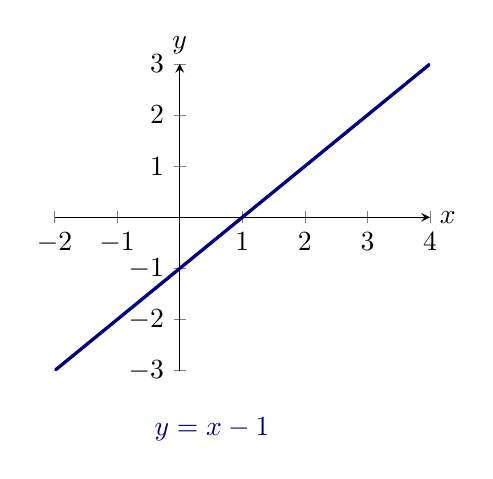
\begin{tikzpicture}
        \begin{axis}[
            domain=-2:4,
            width=2.5in,
            axis lines =middle, xlabel=$x$, ylabel=$y$,
            every axis y label/.style={at=(current axis.above origin),anchor=south},
            every axis x label/.style={at=(current axis.right of origin),anchor=west},
            xtick={-2,...,4},
            ytick={-3,...,3},
          ]
	  \addplot [very thick, penColor, smooth] {x-1};
        \end{axis}
        \node [penColor] at (2,-.75) {$y= x-1$};
      \end{tikzpicture}
      \qquad
      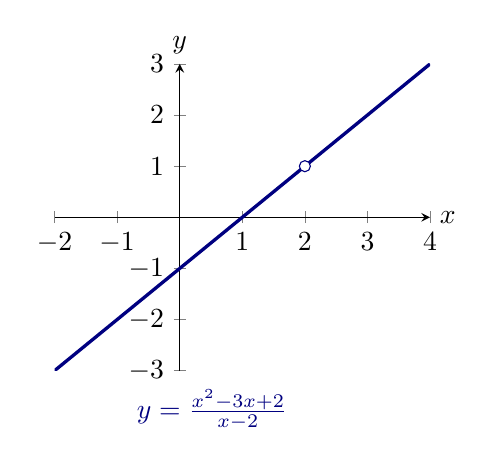
\begin{tikzpicture}
	\begin{axis}[
            domain=-2:4,
            width=2.5in,
            axis lines =middle, xlabel=$x$, ylabel=$y$,
            every axis y label/.style={at=(current axis.above origin),anchor=south},
            every axis x label/.style={at=(current axis.right of origin),anchor=west},
            xtick={-2,...,4},
            ytick={-3,...,3},
          ]
	  \addplot [very thick, penColor, smooth] {x-1};
          \addplot[color=penColor,fill=background,only marks,mark=*] coordinates{(2,1)};  %% open hole
        \end{axis}
        \node [penColor] at (2,-.5) {$y=\frac{x^2-3x+2}{x-2}$};
      \end{tikzpicture}
    \end{image}
    This means that
    \[
    \lim_{x\to 2}\frac{x^2-3x+2}{x-2} = \lim_{x\to 2} (x-1).
    \]
    But now, the limit is in a form on which we can use the limit laws! 
    We have $\lim_{x\to 2} (x-1) =\answer[given]{1}$. Hence
    \[
    \lim_{x\to 2}\frac{x^2-3x+2}{x-2} = \answer[given]{1}.
    \]
  \end{explanation}
\end{example} 


Let's consider some more examples of the form \zeroOverZero.

\begin{example}
  Compute:
  \[
  \lim_{x\to1}\frac{x-1}{x^2+2x-3}.
  \]
  \begin{explanation}
    First note that
    \[
    \lim_{x\to1}\left(x-1\right)=0 \qquad\text{and}\qquad  \lim_{x\to1}\left(x^2+2x-3\right) = 0
    \]
    Hence this limit is of the form \zeroOverZero, which tells us we
    can likely cancel a factor going to $0$ out of the numerator and
    denominator.  Since $\answer[given]{(x-1)}$ is a factor going to $0$ in the
    numerator, let's see if we can factor a $\answer[given]{(x-1)}$ out of the
    denominator as well.
    \begin{align*}
      \lim_{x\to1}\frac{x-1}{x^2+2x-3}&=\lim_{x\to1}\frac{x-1}{(x-1)\answer[given]{(x+3)}} \\
      &=\lim_{x\to1}\frac{1}{\answer[given]{x+3}}\\
      &=\frac{1}{4}.
    \end{align*}
  \end{explanation}
\end{example}


\begin{example}
  Compute:
  \[
  \lim_{x\to 1} \frac{\frac{1}{x+1}-\frac{3}{x+5}}{x-1}.
  \]
\begin{explanation}
  We find the form of this limit by looking at the limits of the
  numerator and denominator separately
  \[
  \lim_{x\to 1}\left(\frac{1}{x+1}-\frac{3}{x+5}\right)=0\qquad\text{and}\qquad\lim_{x\to 1}\left(x-1\right)=0.
  \]
  Our limit is therefore of the form \zeroOverZero\ and we can
  probably factor a term going to $0$ out of both the numerator and
  denominator.
  \[
  \lim_{x\to 1} \frac{\frac{1}{x+1}-\frac{3}{x+5}}{x-1}
  \]
  When looking at the denominator, we hope that this
  term is $(x-1)$.  Unfortunately, it is not immediately obvious how to
  factor an $(x-1)$ out of the numerator.  In order to simplify the
  numerator, we will ``clear denominators.'' by multiplying by
  \[
  1 = \frac{(x+1)(x+5)}{(x+1)(x+5)}
  \]
  this will allow us to cancel immediately
\begin{align*}
  \lim_{x\to 1}& \frac{\frac{1}{x+1}-\frac{3}{x+5}}{x-1}  \cdot \frac{(x+1)(x+5)}{(x+1)(x+5)} \\
  &= \lim_{x\to 1}\frac{(x+5)-3(x+1)}{(x+1)(x+5)(x-1)}.
\end{align*}

Now we will multiply out the numerator.  Note that we do not want to
multiply out the denominator because we already have an $(x-1)$
factored out of the denominator and that was the goal.

\[
\lim_{x\to 1}\frac{(x+5)-3(x+1)}{(x+1)(x+5)(x-1)}
\]
\begin{align*}
  &= \lim_{x\to 1}\frac{x+5-3x-3}{(x+1)(x+5)(x-1)} \\
  &= \lim_{x\to 1}\frac{-2x+2}{(x+1)(x+5)(x-1)}\\
  &= \lim_{x\to 1}\frac{-2\cancel{(x-1)}}{(x+1)(x+5)\cancel{(x-1)}}\\
  &= \lim_{x\to 1}\frac{-2}{(x+1)(x+5)}.
\end{align*}
  
We now have canceled, and can apply the usual Limit Laws.  Hence
\begin{align*}
\lim_{x\to 1} \frac{\frac{1}{x+1}-\frac{3}{x+5}}{x-1}&=\lim_{x\to
  1}\frac{-2}{(x+1)(x+5)}\\
&= \frac{-2}{((1)+1)((1)+5)} \\
&=\answer[given]{\frac{-1}{6}}.
\end{align*}
\end{explanation}
\end{example}

Finally, we'll look at one more example.

\begin{example}
  Compute:
  \[
  \lim_{x\to-1} \frac{\sqrt{x+5}-2}{x+1}.
  \]

\begin{explanation} 
  Note that 
  \[
  \lim_{x\to-1} \left(\sqrt{x+5}-2\right)=0\qquad\text{and}\qquad\lim_{x\to -1} \left(x+1\right) =0.
  \]
  Our limit is therefore of the form \zeroOverZero\ and we
  can probably factor a term going to $0$ out of both the numerator
  and denominator.  We suspect from looking at the denominator that
  this term is $(x+1)$.  Unfortunately, it is not immediately obvious
  how to factor an $(x+1)$ out of the numerator.
 
  We will use an algebraic technique called \dfn{multiplying by the
    conjugate}.  This technique is useful when you are trying to
  simplify an expression that looks like
  \[
  \sqrt{\text{something} \pm \text{something else}}.
  \]
  It takes advantage of the difference of squares rule 
  \[
  a^2-b^2=(a-b)(a+b).
  \]
  In our case, we will use $a=\sqrt{x+5}$ and $b=2$.  Write
  \[
  \lim_{x\to-1} \frac{\sqrt{x+5}-2}{x+1}
  \]
  \begin{align*}
    &= \lim_{x\to-1} \frac{\left(\sqrt{x+5}-2\right)}{(x+1)} \cdot \frac{\left(\sqrt{x+5}+2\right)}{\left(\sqrt{x+5}+2\right)} \\
&=\lim_{x\to-1} \frac{\answer[given]{\left(\sqrt{x+5}\right)^2-2^2}}{(x+1)\left(\sqrt{x+5}+2\right)} \\
&=\lim_{x\to-1} \frac{x+5-4}{(x+1)\left(\sqrt{x+5}+2\right)} \\
&=\lim_{x\to-1} \frac{\cancel{(x+1)}}{\cancel{(x+1)}\left(\sqrt{x+5}+2\right)} \\
&=\lim_{x\to-1} \frac{1}{\sqrt{x+5}+2}\\
&= \frac{1}{\sqrt{-1+5}+2}\\
&=\answer[given]{\frac{1}{4}}.
\end{align*}
\end{explanation}
\end{example}

All of the examples in this section are limits of the form \zeroOverZero.
When you come across a limit of the form \zeroOverZero, you should try
to use algebraic techniques to come up with a continuous
function whose limit you can evaluate.

Notice that we solved multiple examples of limits of the form
\zeroOverZero\ and we got different answers each time.  This tells us
that just knowing that the form of the limit is \zeroOverZero\ is not enough
to compute the limit. The moral of the story is
\begin{center}
  \textbf{Limits of the form \zeroOverZero\ can take any value.}
\end{center}

\begin{definition}
A form that give us no information about the value of the limit is
called an \dfn{indeterminate form}.

A forms that give information about the value of the limit is called a
\dfn{determinate form}.
\end{definition}  

Finally, you may find it distressing that we introduced a form, namely
\zeroOverZero, only to end up saying they give no information on the
value of the limit. But this is precisely what makes
indeterminate forms interesting\dots~they're a mystery!



\end{document}
